\chapter{The Architecture of Dresden OCL2 for Eclipse}
\label{chapter:architecture}

\begin{flushright}
\textit{Chapter written by Claas Wilke}
\end{flushright}

This chapter shortly introduces into the architecture of \acl{DOT4Eclipse}. Before the architecture is presented, some theoretic background is shortly presented.



\section{The Generic Three Layer Metadata Architecture}
\label{architecture:genericLayers}

The \acl{OCL} is a language that is always based on another modeling language (usually the \acs{UML}). Without another language used for modeling, it does not make any sense to define constraints because \acs{OCL} is used for constraint specification but not for modeling itself. Thus, besides \acs{OCL}, a modeling language is required to define a model on that \acs{OCL} constraints can be specified.

Each modeling language is defined in another language, its meta-modeling language. For example, the \acl{UML} is defined using the \keyword{\acf{MOF}} \cite{spec:MOF}, the standardized meta-meta language of the \acs{OMG}. The \acs{MOF} is used to describe the \acs{UML} meta-model that can be used to model \acs{UML} models. Generally spoken, each model requires a meta-model that is used to describe the model. The model can be instantiated by model instances (for example a \acs{UML} class diagram could be instantiated by a \acs{UML} object diagram). The model can be enriched with \acs{OCL} constraints that are defined on the model (using an \acs{OCL} meta-model) and can then be verified for model instances of the model.

The \acs{OMG} introduced the \keyword{\acs{MOF} Four Layer Metadata Architecture} \cite{spec:MOF}\cite[p. 16ff]{spec:UML2-2Inf} that is used to arrange and structure the meta-model, the model, and its model instances into a layered hierarchy (see Figure \ref{pic:architecture:mofLayers}; the layout of the illustration is oriented at the conceptual framework introduced by Matthias Br�uer \cite[p. 28]{GB:Braeuer}). Generally, four layers exist, the \keyword{Meta-Meta-Model Layer (M3)}, the \keyword{Meta-Model Layer (M2)}, the \keyword{Model Layer (M1)}, and the \keyword{Model Instance Layer (M0)}.

\begin{figure}[!p]

	\centering
	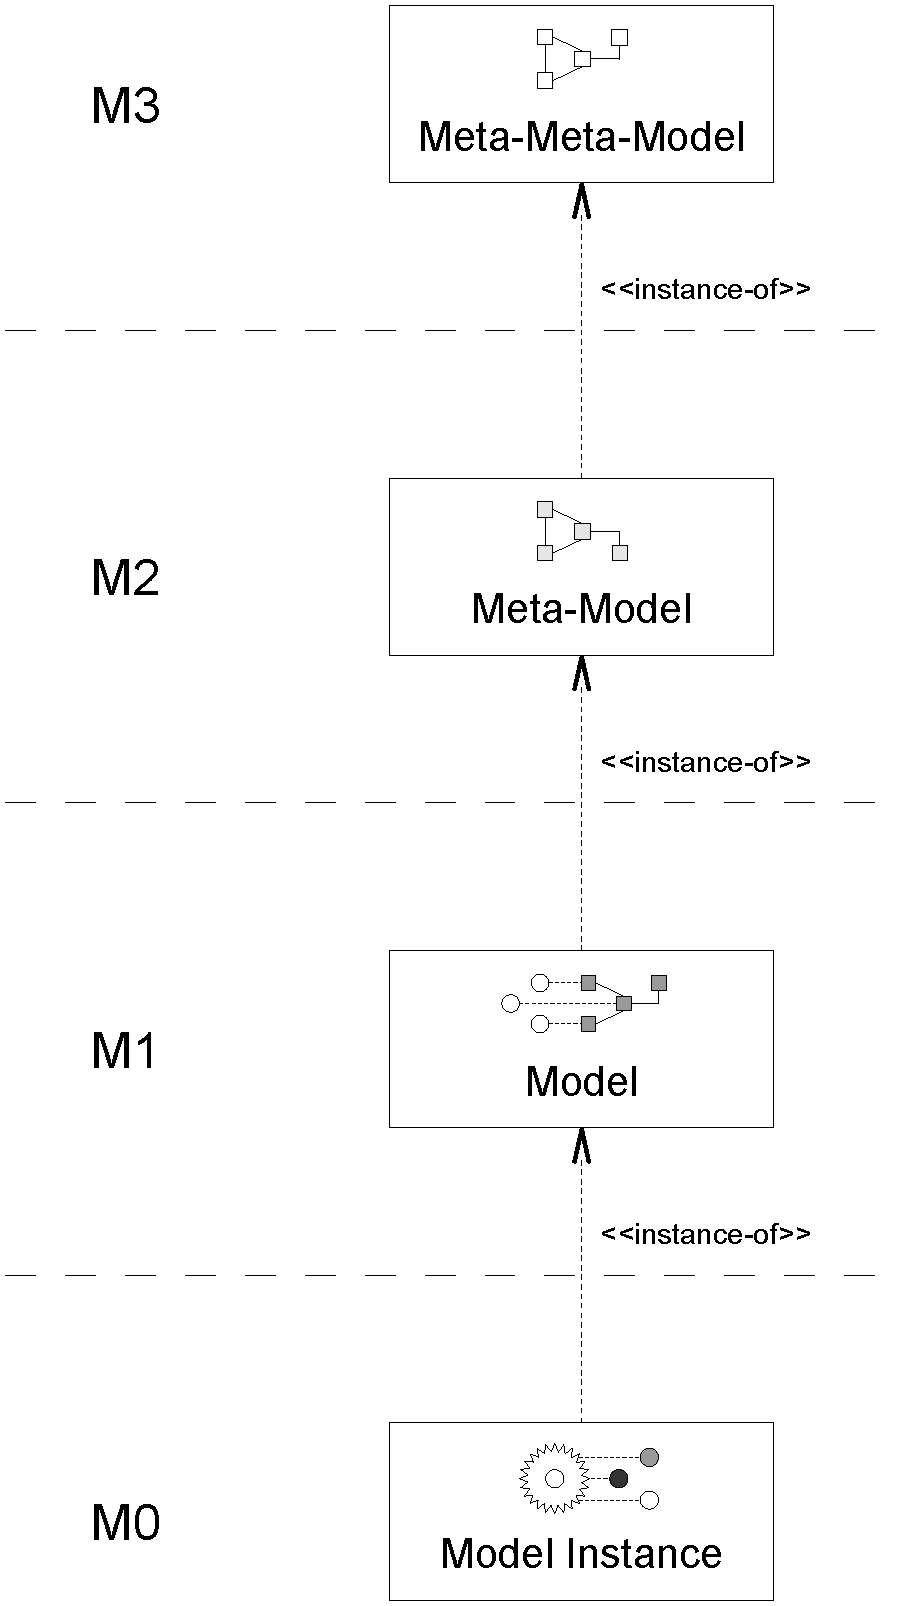
\includegraphics[width=.4\linewidth]{figures/architecture/mofLayers}
	\caption{The MOF Four Layer Metadata Architecture.}
	\label{pic:architecture:mofLayers}

  \vspace{4.5em}
  
	\centering
	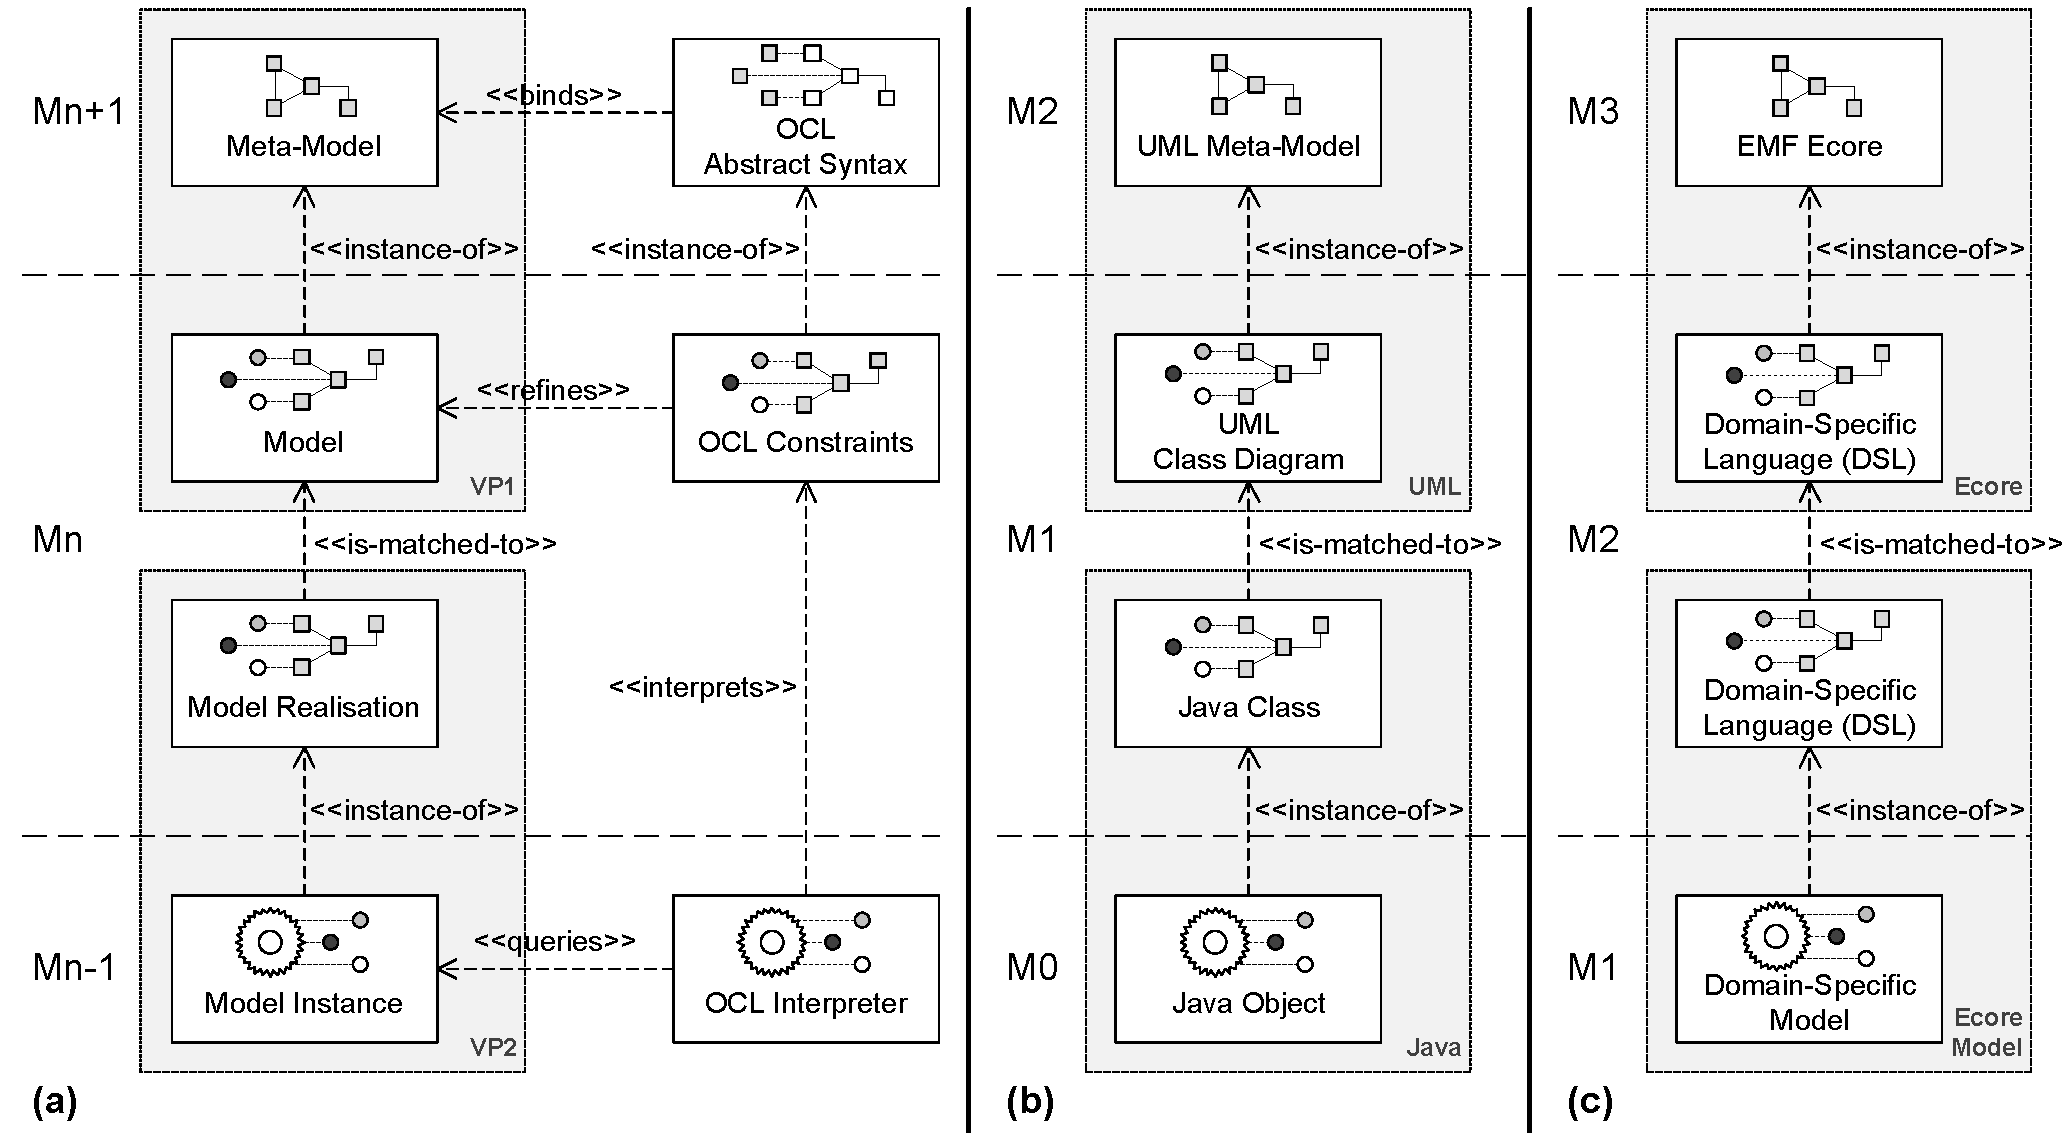
\includegraphics[width=.4\linewidth]{figures/architecture/genericLayers}
	\caption{The Generic Three Layer Metadata Architecture.}
	\label{pic:architecture:genericLayers}

\end{figure}

\acs{OCL} constraints can be defined on both, meta-models and models to verify models respectively model instances. Thus, the four layer metadata architecture can be generalized to a \keyword{Generic Three Layer Metadata Architecture} in the scope of an \acs{OCL} definition (see Figure \ref{pic:architecture:genericLayers}) \cite{demuth:RGWS09}. On the \keyword{Mn+1 Layer} lies the meta-model that is used to define the model that shall be constrained. On the \keyword{Mn Layer} lies the model that is an instance of the meta-model and can be enriched by the specification of \acs{OCL} constraints. Finally, on the \keyword{Mn-1 Layer} lies the model instance on that the \acs{OCL} constraints shall be verified. Please note, that in the context of such a generic layer architecture, a model
instance can be both a model (like a \acs{UML} class diagram) or a set of objects (like Java run-time objects). 



\section{The Toolkit's Architecture}

The architecture of \acl{DOT4Eclipse} is shown in Figure \ref{pic:architecture:modules}. The architecture is the result of the work of Matthias Br�uer \cite{GB:Braeuer} and can easily be extended. The architecture can be separated into three layers: The \keyword{Back-End}, the \keyword{Basis} and the \keyword{Tools Layer}.

\begin{figure}[!htbp]

	\centering
	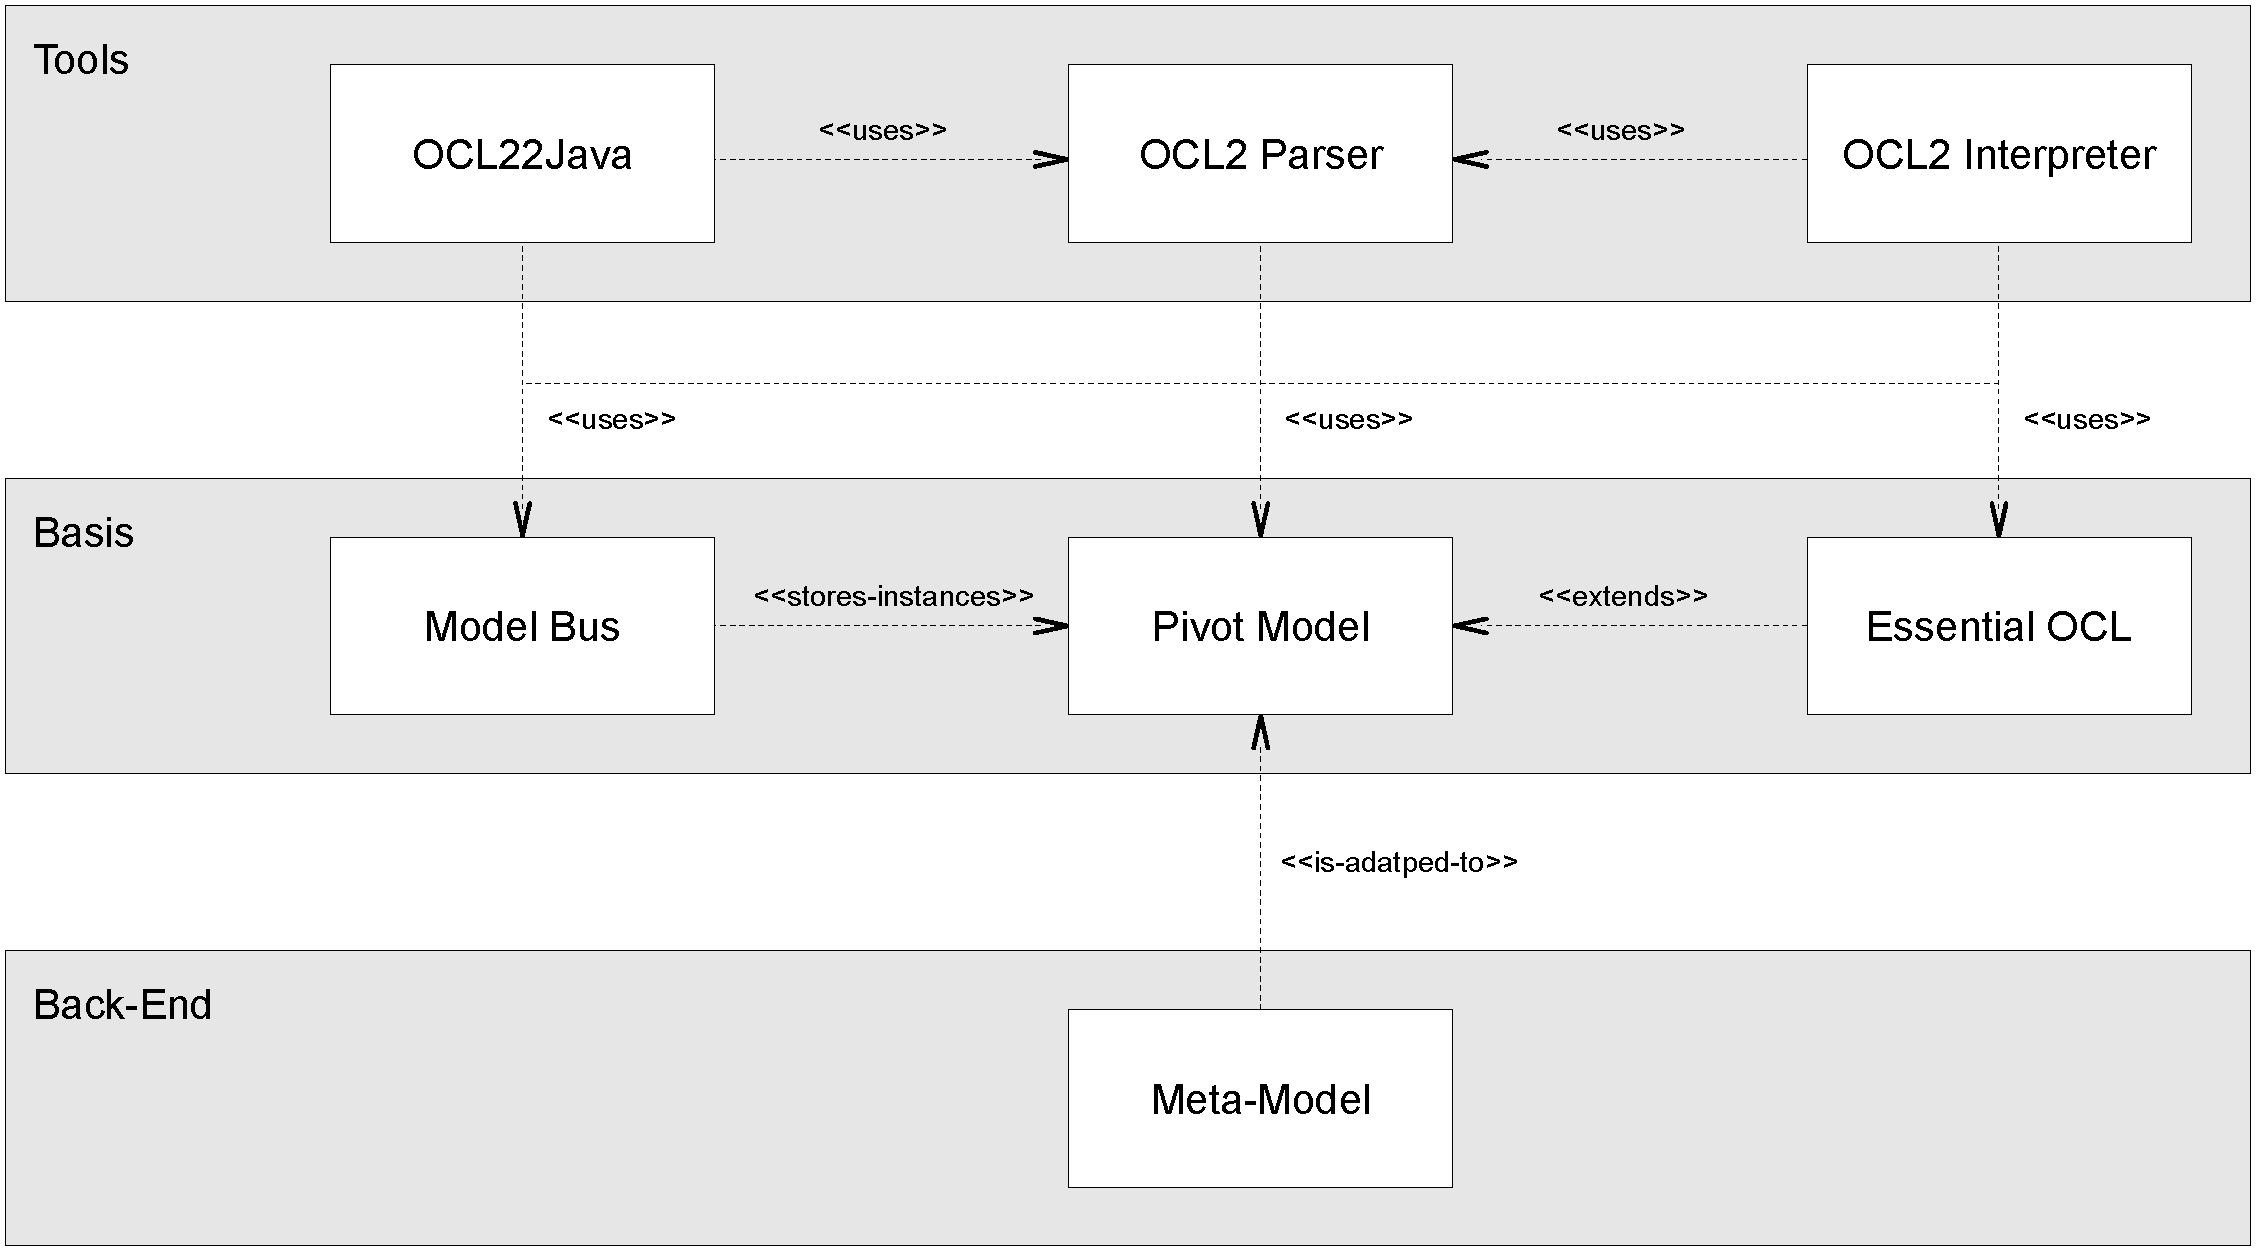
\includegraphics[width=1.0\linewidth]{figures/architecture/modules}
	\caption{The architecture of Dresden OCL2 for Eclipse.}
	\label{pic:architecture:modules}

	\vspace{6.5em}
	
	\centering
	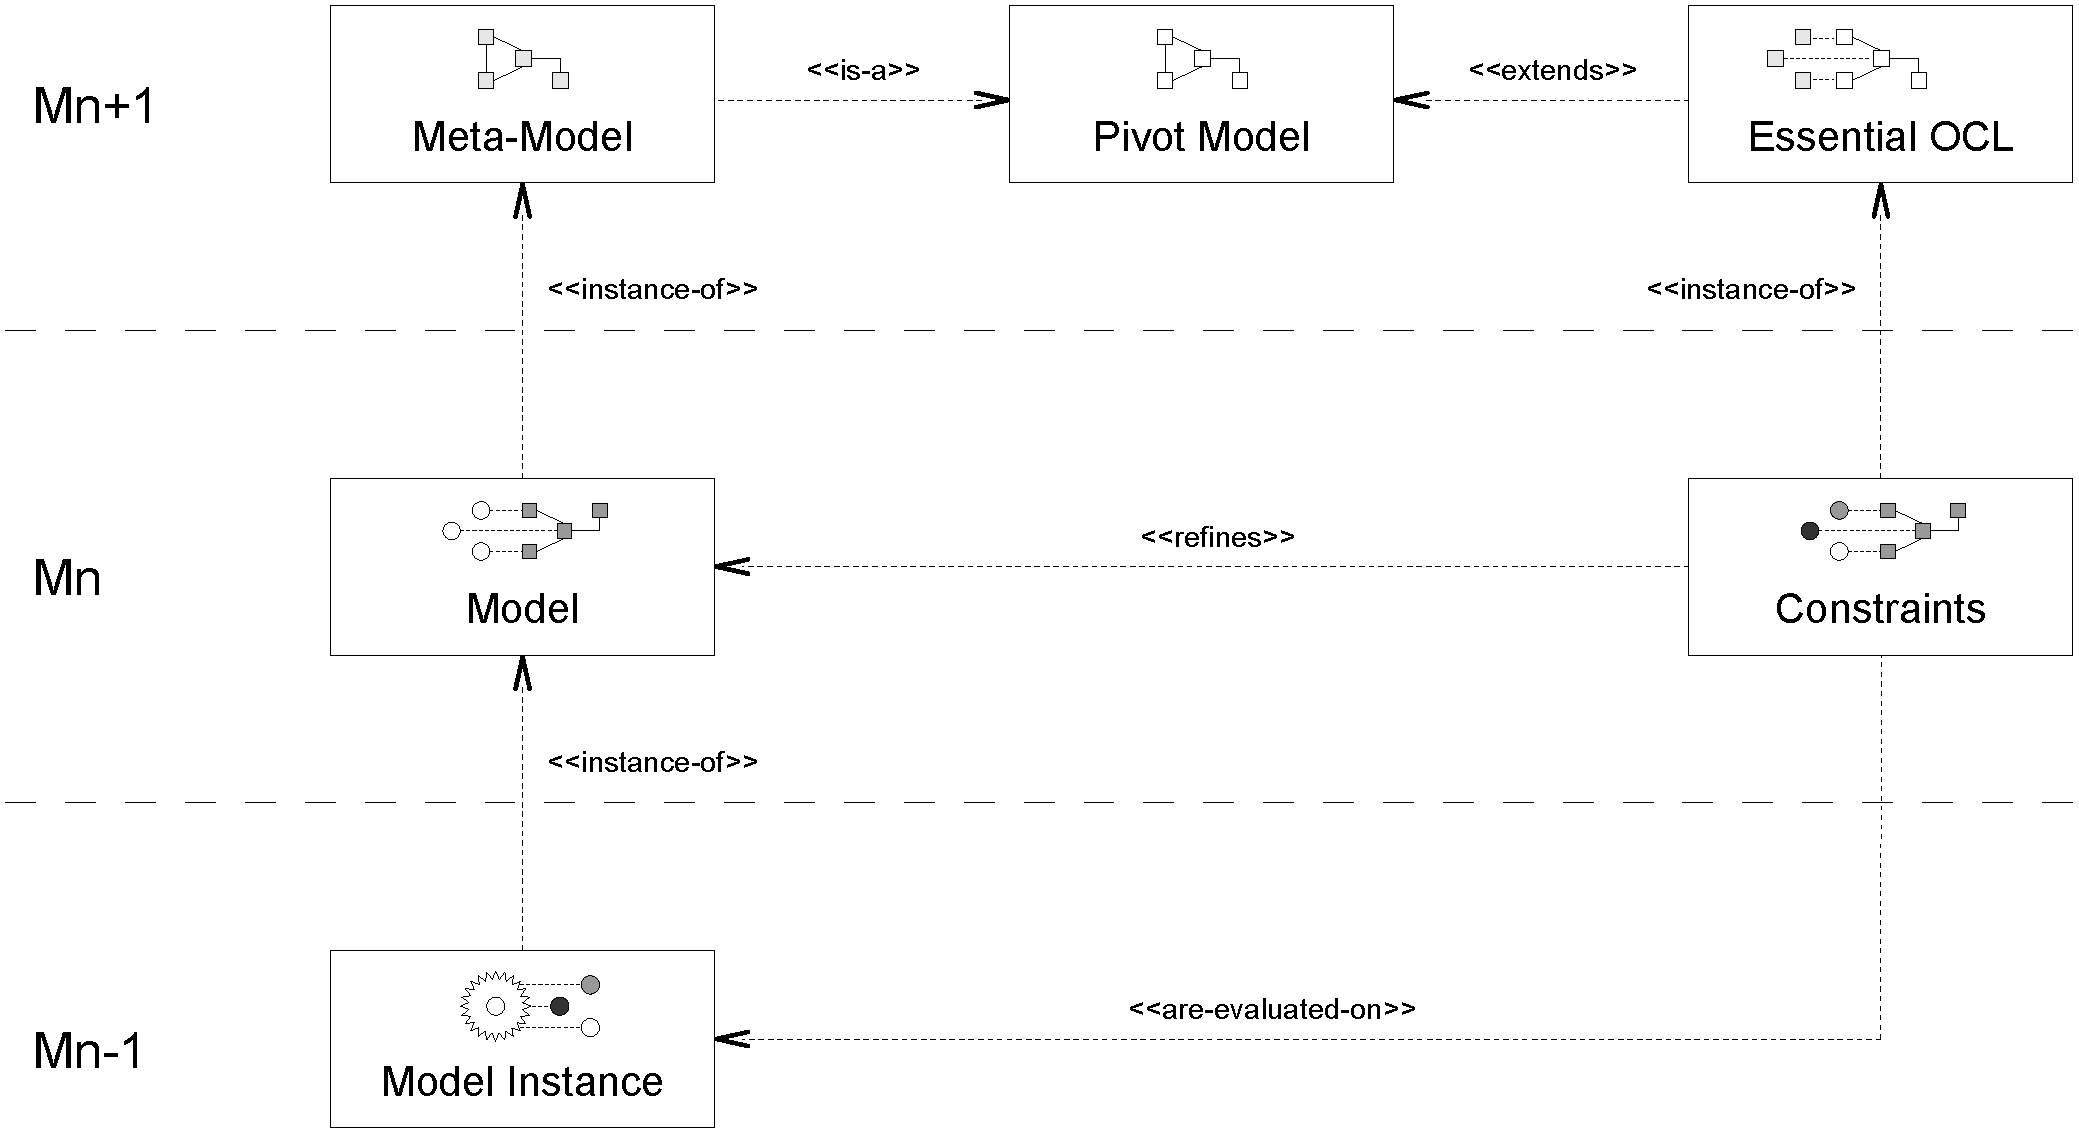
\includegraphics[width=1.0\linewidth]{figures/architecture/genericArchitecture}
	\caption{The architecture of Dresden OCL2 for Eclipse in respect to the Generic Three Layer Metadata Architecture.}
	\label{pic:architecture:genericArchitecture}

\end{figure}

The back-end layer represents the repository and the meta-model which can easily be exchanged because all other packages of  \acl{DOT4Eclipse} do not directly communicate with the meta-model but use the \keyword{Pivot Model} that delegates all requests to the meta-model instead. For example a possible meta-model is the \acs{UML}2 meta-model of the \keyword{\acf{Eclipse MDT} Project} \cite{WWW:MDT}. The second layer is the toolkit basis layer and contains the \keyword{Pivot Model}, \keyword{Essential OCL} and the \keyword{Model Bus}. The use of the pivot model was explained before. The package \keyword{Essential OCL} extends the pivot model and implements the \keyword{\acs{OCL} Standard Library} to extend loaded models with \acs{OCL} constraints. The package \keyword{Model Bus} loads, manages and provides access to models the user wants to work with. The third layer contains all tools that are provided by the toolkit. This layer contains the \keyword{\acs{OCL}2 Parser} (which is essential, because the other tools require models that are enriched with already parsed and syntactically and semantically checked constraints), the \keyword{\acs{OCL}2 Interpreter},  and the \keyword{\acs{OCL}22Java Code Generator}. All the tools use the packages of the second layer to access models and model instances and to work on \acs{OCL} constraints.

\acl{DOT4Eclipse} has been developed as a set of Eclipse/\acs{OSGi} plug-ins. All packages that are located in the basis and tools layer represent different Eclipse plug-ins. Additionally, \acl{DOT4Eclipse} contains some plug-ins to provide \acs{GUI} elements such as wizards and examples to run \acl{DOT4Eclipse} with some simple models and \acs{OCL} expressions.

\subsubsection{\acl{DOT4Eclipse} and The Generic Three Layer Metadata Architecture}
\label{theory:DOTLayers}

The architecture of \acl{DOT4Eclipse} was designed in respect to the Generic Three Layer Metadata Architecture (introduced in Section \ref{architecture:genericLayers}, see Figure \ref{pic:architecture:genericArchitecture}). At the \keyword{Mn+1 Layer}, different meta-models and \acs{DSL}s can be adapted to the toolkit by adapting them to the pivot model (as explained in Chapter \ref{chapter:pivotModelAdaptation}. Afterwards, models defined with the elements of these meta-models can be loaded into the toolkit at the \keyword{Mn Layer}. The models can be enriched with \acs{OCL} constraints that are described using their own meta-model, Essential \acs{OCL}, which is described at the \keyword{Mn+1 Layer} by extending the pivot model. At the \keyword{Mn-1 Layer} model instances of models loaded before can be imported into the toolkit and \acs{OCL} constraints can be verified on these model instances by using the \acs{OCL}2 Interpreter or the \acs{OCL}22Java Code Generator. Please note that model instances can be both, models like \acs{UML} class diagrams or model instances like Java objects.